%%=============================================================================
%% Conclusie
%%=============================================================================
\chapter{Conclusie}%
\label{ch:conclusie}


Google Cloud Platform is zeker niet geschikt voor deze specifieke use-case, we moeten dus enkel nog Azure en AWS vergelijken. Hiervoor zullen we kijken naar de gelijkenissen, verschillen en resultaten van de modellen die de 2 providers hebben gegenereerd. 

\section{Gelijkenissen}
De grootste gelijkenis zijn de stappen die nodig zijn om een MLaaS instantie op te zetten. In beide gevallen wordt er ook een data-opslag service opgestart waar zowel de input-data in kan worden opgeslaan als de output-data naar kan worden weggeschreven. Beide providers laten ook toe om modellen te deployen via een hun eigen Infrastructure as a Service (IaaS). 

\section{Verschillen}
Een eerste verschil is dat AWS meerdere bestands-types ondersteunt dan Azure (dat alleen CSV-bestanden ondersteunt), Azure ondersteunt dan weer meerdere programmeer talen en Machine Learning frameworks. Alhoewel beide providers werken met een pay-as-you go systeem, is er bij Azure de mogeljikheid om te configureren op welke virtuele machine de training jobs moeten worden uitgevoerd, waardoor er meer flexibiliteit is en het totale kostenplaatje goedkoper kan worden geconfigureerd bij Azure. Zoals eerder vermeld kunnen beide providers modellen ook deployen, maar alleen Azure laat toe om de modellen te exporteren naar een lokaal werkende instantie.
Ten slotte bieden beide providers een standaard dataset aan die kan gebruikt worden om te experimenteren met de mogelijkheden van de MLaaS. AWS SageMaker biedt ook theoretische documenten aan om de interne werking van de processen uit de doeken te doen, terwijl Azure meer documentatie aanbiedt over het gebruik van de effectieve services. 


\section{Resultaten}
Het is duidelijk dat Azure betere resultaten kan voorleggen voor deze use-case dan AWS, zowel de nauwkeurigheid \ref{nauwkeurigheid_chart} als de gewogen nauwkeurigheid \ref{gewogen_nauwkeurigheid_chart} zijn voor alle data-sets hoger.  
\begin{figure}[h]
    \caption{Bar chart die de nauwkeurigheden van AWS en Azure vergelijkt per percentage van de dataset dat werd gebruikt als trainingsdata.}
    \centering
    \label{nauwkeurigheid_chart}
    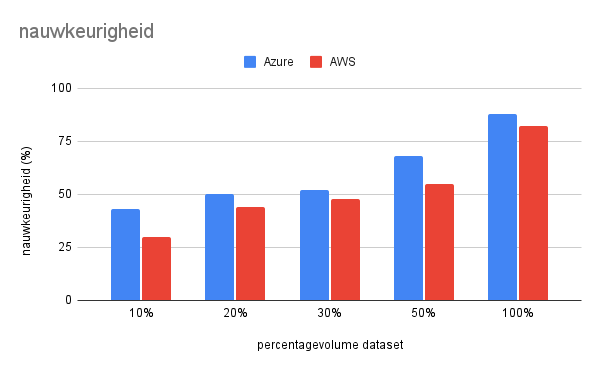
\includegraphics[width=0.75\textwidth]{nauwkeurigheid}
\end{figure}

\begin{figure}[h]
    \caption{Bar chart die de gewogen nauwkeurigheden van AWS en Azure vergelijkt per percentage van de dataset dat werd gebruikt als trainingsdata.}
    \centering
    \label{gewogen_nauwkeurigheid_chart}
    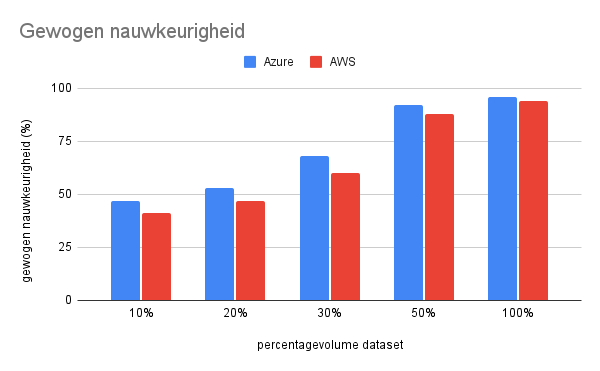
\includegraphics[width=0.75\textwidth]{Gewogen nauwkeurigheid}
\end{figure}

De gewogen nauwkeurigheid bereikt reeds 92\% wanneer 50\% van de originele dataset wordt gebruikt als trainingsdataset. 

\section{Beslissen}
\subsection{Proof of Concept}
De eerste vraag die moet worden gesteld is of de modellen die zijn gegenereerd überhaupt zouden kunnen helpen bij het on-boarding proces van een nieuw PIM-systeem. Het is duidelijk dat voor beide providers de modellen die gegeneerd werden op basis van de datasets die respectievelijk 10\%, 20\% en 30\% van de originele dataset bevatten, zeker niet geschikt zijn voor het autonoom toevoegen van tags aan de entiteiten van het systeem. Zowel het model van Azure als het model van AWS die met 50\% (350 records) van de originele dataset werden gegenereerd zijn zeker geschikt voor het geven van gerichte suggesties, en eventueel ook al voor het zelfstandig taggen van entiteiten. Beide modellen die werden gegenereerd met de originele dataset zijn zeker geschikt voor het geven van suggesties en ook voor het zelfstandig taggen. Dit wil zeggen dat het integreren van Machine Learning in het taxonomie systeem van PIMLayer zou kunnen helpen bij zowel het onboarding proces als bij het onderhouden en updaten van een bestaand PIM-systeem. Dat laatste is ook interessant voor andere PIM-systemen, zoals het systeem waar de Constructalia-dataset werd uit gehaald. 
\subsection{AWS of Azure}
Voorlopig gebruikt PIMLayer geen specifieke AWS of Azure producten. De snelheid van de services van de providers spelen in deze geen rol, aangezien het vaak gaat over buffer operaties met een lage prioriteit (zeker in het onboarding proces). Dat wil zeggen dat we ons kunnen beperken tot de resultaten en de prijs om een beslissing te nemen tussen beide providers. 
Aangezien Azure betere resultaten kan neerleggen voor elke train-dataset en er een goedkopere configuratie kan worden gemaakt op Azure is de keuze voor Azure de logische. 


\section{Toegevingen}
\subsection{1 model per tag}
De modellen die in dit onderzoek worden gegenereerd kunnen slechts 1 tag voorspellen, terwijl PIMLayers tag-systeem meerdere soorten tags ondersteunt. Dit wil zeggen dat er voor elke tag een ander model zou moeten worden gegenereerd, en dat ook nog eens voor elke klant. Het zou dan ook interessant kunnen zijn om de eindgebruiker te laten instellen voor welk type tags er een model moet worden voorzien en voor welke niet.

\subsection{Meerdere tags binnen dezelfde groep}
Het taxonomie systeem van PIMLayer ondersteunt ook meerdere tags per bestand, de modellen die voor dit onderzoek zijn gegenereerd konden hier moeilijk mee om, zo bleek uit de zoektocht naar welke tag de modellen zouden moeten gaan voorspellen. Misschien is het mogelijk om de gegeneerde modellen zodanig aan te passen opdat ze hier wel mee kunnen omgaan.  

\subsection{Negatieve feedbackloop}
Hoe kan ervoor worden gezorgd dat het model blijft bijleren? Zou het mogelijk zijn om een negatieve feedbackloop toe te voegen aan de modellen zodat het voorspellend vermogen van een model toeneemt? 

\section{Verder onderzoek}
Nu er een keuze kan gemaakt worden qua provider is de volgende uitdaging om deze te integreren in PIMLayer zelf. Er moet ook nog nagedacht worden over hoe en op welke manier dit zou moeten gebeuren...

% TODO: Trek een duidelijke conclusie, in de vorm van een antwoord op de
% onderzoeksvra(a)g(en). Wat was jouw bijdrage aan het onderzoeksdomein en
% hoe biedt dit meerwaarde aan het vakgebied/doelgroep? 
% Reflecteer kritisch over het resultaat. In Engelse teksten wordt deze sectie
% ``Discussion'' genoemd. Had je deze uitkomst verwacht? Zijn er zaken die nog
% niet duidelijk zijn?
% Heeft het onderzoek geleid tot nieuwe vragen die uitnodigen tot verder 
%onderzoek?



